\newpage
\section{Auswertung}
\label{sec:Auswertung}
\subsection{Eichung des Magnetfeldes}
Die bei der Messung aufgenommenen Magnetfeldstärken $B$ bei angelegter Stromstärke $I$ befinden sich in Tabelle \ref{tab:bfeld}.

\begin{table}
    \centering
    \sisetup{table-format=2.1}
    \begin{tabular}{c c}
    \toprule
    $I \,/\,A$ & $B \,/\, mT$ \\
     \midrule 
  0  & 7.6  \\
  0.5  & 60  \\
  1  & 105.6   \\
  1.5  & 154.1  \\
  2  & 202.3   \\
  2.5  & 255.1  \\
  3  & 298.6   \\
  3.5  & 339.1  \\
  4  &  386.2   \\
  4.5  &  421.3 \\
  5  & 455.7 \\
    \bottomrule
    \end{tabular}
    \caption{Messwerte der Magnetfeldstärke in Abhängigkeit der Stromstärke.}
    \label{tab:bfeld}
    \end{table}


\noindent
Die Messwerte werden mittels python an eine Funktion dritten Grades gefittet.
Für die Fitfunktion

\begin{equation*}
    B(I)=aI^3 + bI^2 + cI + d
\end{equation*}

\noindent
werden die folgenden Parameter ermittelt:

\begin{align*}
    a&=-0.78 \pm 0.25 \, \frac{\text{mT}}{\text{A}^3} \\
    b&=2.70  \pm 1.90 \, \frac{\text{mT}}{\text{A}^2} \\
    c&=95.34 \pm 3.97 \, \frac{\text{mT}}{\text{A}} \\
    d&=8.90  \pm 2.18 \, \text{mT} \\
\end{align*}

\noindent
Die Messwerte und die Ausgleichskurve sind in Abbildung \ref{fig:bfeld} dargestellt.

\begin{figure}
    \centering
    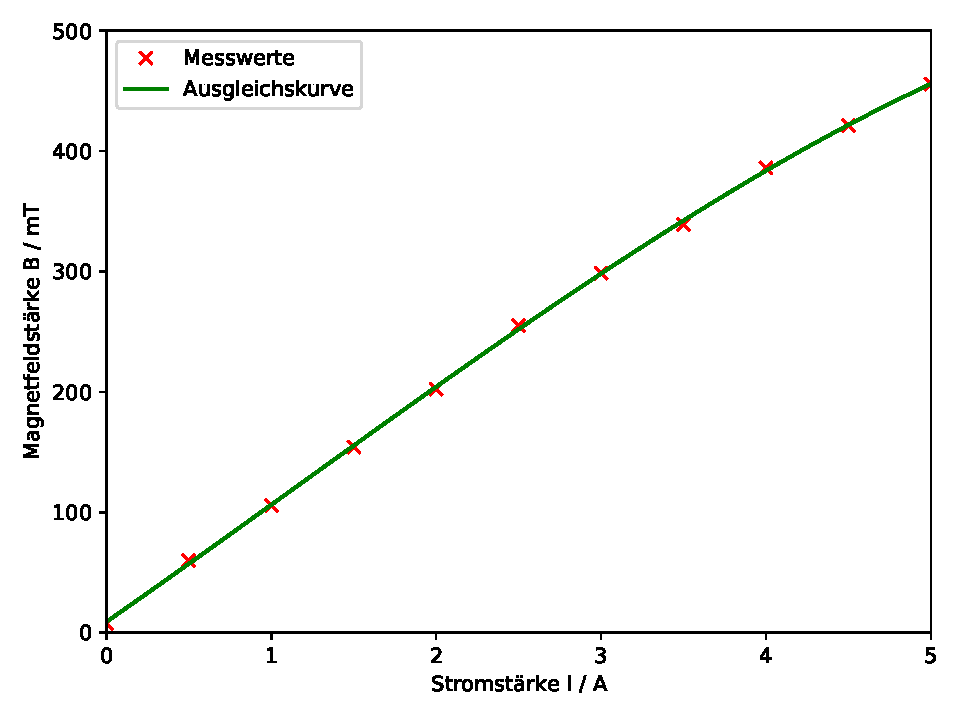
\includegraphics[width=0.75\textwidth]{data/Magnetfeld.pdf}
    \caption{Ausgleichskurve durch die Messwerte der Magnetfeldstärke.}
    \label{fig:bfeld}
  \end{figure}

\subsection{Rote Spektrallinie}